\chapter{Simulation Structure}\label{simulation_structure}

%%%%%%%%
%%%%%%%% Simulation Environment
%%%%%%%%
\section{Simulation Environment}\label{simulation_environment}
Goes over the backend design

%%%%%%%%
%%%%%%%% Simulation Flow
%%%%%%%%
\section{Simulation Flow}\label{simulation_flow}
The order in which events happen
Need a nice diagram for this

%%%%%%%%
%%%%%%%% Message Passing
%%%%%%%%
\section{Message Passing}\label{message_passing}
Need a nice diagram for this

%%%%%%%%
%%%%%%%% Health Modeling
%%%%%%%%
\section{Health Modeling}\label{health_modeling}

%
%%%%%%%% Global Description
%
\subsection{Global Description}

The health of the agents living in the tower is represented by Health Points (HP). Two mechanisms affect an agent's HP: how much food they eat, and their ``cost of living''. The cost of living represents how many calories a human needs to eat each day to stay healthy. These two mechanisms are implemented using the functions \lstinline$updateHP$ and \lstinline$hpDecay$, respectively. These two functions are described below.

At the end of each day, agents are assigned an HP value based on how much food they have eaten and their cost of living. This HP value is an integer and has a maximum value of \lstinline$MaxHP$, and a minimum value of \lstinline$HPCritical$. As its name suggests, \lstinline$HPCritical$ is a critical HP value for the agents: they can only survive a certain number of days (\lstinline$MaxDayCritical$) at this level. When in the critical state, if agents can increase their HP by \lstinline$HPReqCToW$ (``HP Required to move from Critical To Weak''), then they move into the \lstinline$WeakLevel$ (\Cref{fig:health_system}), and their HP takes the value of \lstinline$WeakLevel$. The amount that an agent's HP increases from eating is determined by the function \lstinline$updateHP()$.

\begin{figure}[htb]
    \centering
    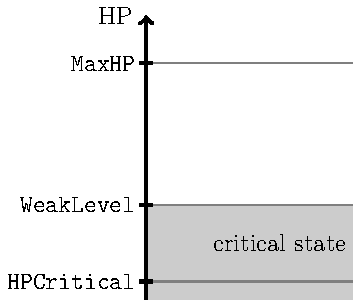
\includegraphics[width=0.3\linewidth]{002_simulation_structure/images/health_global.pdf}
    \caption{The health of the agents is represented by a HP value between \lstinline$HPCritical$ and \lstinline$MaxHP$. All HP values which are below \lstinline$WeakLevel$ are classed as critical. The diagram is not drawn to scale.}
    \label{fig:health_system}
\end{figure}

\subsection{Food and Health: \texorpdfstring{\texttt{updateHP}}{updateHP}}\label{updateHP}
To increase their HP, agents need to eat. However, the amount an agent's HP improves can saturate in a single day; eating more than a certain amount will provide an agent with no extra benefit to their HP. Moreover, eating more food will lead to diminishing returns in terms of HP change. Mathematically, the ideas of diminishing returns and saturation are well captured by the step response of a 1st-order system \eqref{updateHP_general}:

\begin{equation}\label{updateHP_general}
   \texttt{newHP}= \texttt{currentHP} +\underbrace{w(1-e^{\frac{-\texttt{foodTaken}}{\tau}})}_{\texttt{HPChange}}
\end{equation}

The two parameters $w$ and $\tau$ are defined at the beginning of the simulation. The shape of this curve is given in \Cref{fig:updateHP} together with some important parameters.

\begin{figure}[htb]%
    \centering
    \subfloat[\centering Overview]{{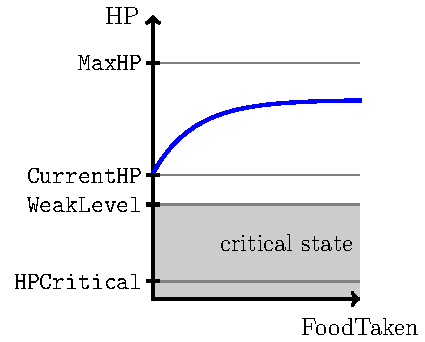
\includegraphics[width=0.36\linewidth]{002_simulation_structure/images/health_updateHP_overview.pdf}}}%
    \qquad
    \subfloat[\centering Detailed representation]{{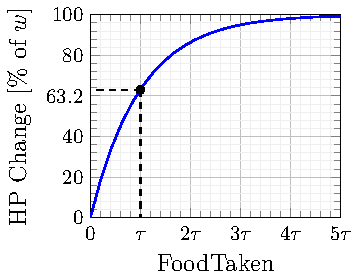
\includegraphics[width=0.36\linewidth]{002_simulation_structure/images/health_updateHP_detailed.pdf}}}%
    \caption{\texttt{updateHP} as a function of the amount of food eaten (``FoodTaken'').}%
    \label{fig:updateHP}%
\end{figure}

It is not possible to gain more HP than $w$ over the duration of one day; this is an intentional limit to prevent an agent's health from improving too quickly. As an example, we can think of an agent that starts from the weak level and wants to reach the maximum HP value. It would take several days for this agent to ``recover'' from this weak level and stabilise its health to a high HP value. 

Note that it is possible for an agent to achieve an HP value that is larger than \texttt{MaxHP} inside \lstinline$hpDecay$. At the end of each day, the \lstinline$hpDecay$ function will apply the cost of living and then bound the final HP value by \lstinline$MaxHP$.


Agents in the critical state are treated differently. For these agents, HP is updated according to equation \eqref{updateHP_critical}:

\begin{equation}\label{updateHP_critical}
    \texttt{newHP} = \min\left\{\texttt{HPCritical}+\texttt{HPReqCToW}, \texttt{currentHP} +w(1-e^{\frac{-\texttt{foodTaken}}{\tau}})\right\}
\end{equation}

\subsection{Cost of Living: \texorpdfstring{\texttt{hpDecay}}{hpDecay}}\label{hpDecay}
At the end of each day, the HP value of the agents will be reduced by the cost of living. The cost of living is larger for an agent with larger HP value than for an agent with lower HP value. This fact is motivated by a simple observation: humans that have stronger bodies and immune systems also need more food to sustain their level of health. The exact relation between HP value, cost of living, and HP value after applying the cost of living is given by the linear relation \eqref{hpDecay_equation}:

\begin{equation}\label{hpDecay_equation}
    \texttt{newHP} = \texttt{currentHP}-\left[b + s(\texttt{currentHP}-\texttt{WeakLevel})\right]
\end{equation}


The parameter $b$ is a (constant) base cost, and $s$ is the slope of the linear function. These parameters are initialised at the beginning of the simulation.

To ensure that the HP value at the end of the day is bounded by \texttt{MaxHP}, we slightly modify (\ref{hpDecay_equation}) to produce (\ref{hpDecay_bounded}):

\begin{equation}\label{hpDecay_bounded}
    \texttt{newHP} =\max\left\{\texttt{MaxHP}, \texttt{currentHP}-\left[b + s(\texttt{currentHP}-\texttt{WeakLevel})\right]\right\}
\end{equation}

For agents in the critical state that gain \texttt{HPReqCToW} HP in a single day, i.e. their HP after eating is

\begin{equation}\label{HPReqCToW}
    \texttt{currentHP} \geq \texttt{HPCritical}+\texttt{HPReqCToW},
\end{equation}

their HP will be set to \texttt{WeakLevel}. Agents in the critical state which do not manage to improve their HP by \lstinline$HPReqCToW$ will be kept in the critical state:

\begin{equation}\label{hpDecay_critical_stay}
    \texttt{newHP} = \texttt{HPCritical}
\end{equation}

with the \texttt{daysAtCritical} counter incremented by 1. If \texttt{daysAtCritical} reaches \texttt{MaxDayCritical}, the agent dies and is replaced. This counter is reset to 0 if an agent exits the critical state.




%%%%%%%%
%%%%%%%% Global Utility
%%%%%%%%
\section{Utility and Social Welfare}\label{utility}

To assess the performance of the agents in the tower as a group, we first need to define a metric. A common choice is the so-called \emph{social welfare}, based on each agent individual utility. For this project, we implement the notion of utility as introduced in \cite{somasPitt}.

Our system is composed of $N$ agents that can perform specific actions in relation with the common pool resources. In a general context, each agent 
$i\in\{1, \ldots, N\}$ takes the following actions at each iteration $t\in\{1,\ldots,\infty\}$:

\begin{enumerate}
    \item Determines the resources it has available, $g_i \in [0,1]$.
    \item Determines its need for resources, $q_i \in [0,1]$.
    \item Makes a provision of resources, $p_i \in [0,1]$.
    \item Makes a demand for resources, $d_i \in [0,1]$.
    \item Receives an allocation of resources, $r_i \in [0,1]$.
    \item Makes an appropriation of resources, $r'_i \in [0,1]$.
\end{enumerate}

In the current setup, the available resources $q_i$ corresponds to the current amount of food on the platform.  The need for resources $q_i$ is defined in relation with the health of the agents. We set the following values to $q_i$:

\begin{equation}\label{resources_needed}
    q_i=\begin{cases}
     \frac{\texttt{numberDaysInCriticalState}}{\texttt{maxDaysInCriticalState}} & \mbox{if } \texttt{currentHP}\leq \texttt{weakLevel}  \\ 
     0 & \mbox{else.}
     \end{cases}
\end{equation}

This way, we ensure that $q_i$ is bounded by 1 and is proportional to the days spent in the critical health zone below \texttt{weakLevel}.

Moreover, the agents do not make any provision $p_i$ to the common pool, as they cannot give food to the platform ($p_i=0$). Their demands for resources is the food they ask for when the platform is at their level. In addition, the agents appropriate all resources they are allocated, so that $r'_i=r_i$.\footnote{We ensure that all these parameters are constrained to the range $[0,1]$ by dividing the mentioned quantities by their maximum values.}

The total resources accrued at the end of an iteration, $R_i$, is hence defined as:

\begin{equation}\label{resources_accrued}
    R_i=r'_i+ (g_i-p_i)
\end{equation}

where each agent will `generate' resources equal to: its appropriation, plus the amount available on the platform, minus the provision made back to the common pool.

Using the above parameters, it is possible to compute the following utility per agent:

\begin{equation}\label{utility_per_agent}
    u_i=\begin{cases}
     \alpha_iq_i + \beta_i(R_i-q_i) & \mbox{if } R_i\geq q_i  \\ 
     \alpha_i R_i - \gamma_i(q_i-R_i) & \mbox{else}
     \end{cases}
\end{equation}


where $\alpha_i$, $\beta_i$ and $\gamma_i$ are tuning parameters that follow the rule $\alpha_i>\gamma_i>\beta_i$. In our work, we use the values $\alpha_i=\alpha=0.2$, $\beta_i=\beta=0.1$, and $\gamma_i=\gamma=0.18$.

Finally, we use \eqref{utility_per_agent} to compute an average global utility, which corresponds to the social welfare \textit{SW} divided by the number of agents:

\begin{equation}\label{utility_eq}
    \mathit{U}=\frac{\sum_i^N u_i}{N}=\frac{\mathit{SW}}{N}
\end{equation}